
	
	\noindent \section{Problem 1} 

Finding a good biochemical marker for fat intake is an important problem in cancer
							prevention research. The total cholesterol level or derivative measures such as HDL and
							LDL are normally used. However, it is well known that these measures are highly variable
							within an individual and, therefore, may not be reliable measures of fat intake. Many
							studies have shown that carnitine, a betaine derivative, C7H15NO3, may be useful as an
							alternative biochemical marker for fat intake. \\
							
							\vspace{0.2cm} 
	\noindent  	To investigate the effectiveness of carnitine as a biochemical marker for fat intake, a
							randomized experiment was conducted on 14 female monkeys. During an initial run-in
							period of 12 weeks all monkeys were put on a high, exclusively polyunsaturated, fat diet
							to stabilize their carnitine levels (data not included). After the run-in period, monkeys were randomized to
							two groups. Those monkeys randomized to group 1 received a low, exclusively polyunsaturated,
							fat diet, while those in group 2 continued on the same diet as in the run-in period.
							At week 10 after randomization, the polyunsaturated fat was replaced by saturated fat in
							both groups, with those in group 1 receiving a low saturated fat diet and those in group
							2 receiving a high saturated fat diet. Thus, in the current design, there are two levels of
							fat in the diet, high fat and low fat, and two types of fat, saturated and polyunsaturated. \\
				
							\vspace{0.2cm} 
	\noindent 	Weekly measurements of total plasma carnitine were obtained starting the week of randomization.
							Measurements at weeks 10 through 15 post randomization were not taken
							because that period was considered a “washout” period. In other words, measurements
							were made at weeks 1-9 and weeks 16-30. The goal of the current analysis is to investigate
							the relationship between fat and carnitine. \\
				
							\vspace{0.2cm} 
	\noindent  	The file \texttt{monkey.dat} contains the following variables:
							\begin{itemize}
								\item id: animal id number
								\item group: group number (1=low fat diet; 2=high fat diet)
								\item cartn0: total carnitine (nmol/ml) at randomization (baseline carnitine measure)
								\item cartn1: total carnitine (nmol/ml) 1 week after randomization \\
								 \vspace{0.2cm} ...
								\item cartn30: total carnitine (nmol/ml) 30 weeks after randomization
							\end{itemize}
				
				
				
							\begin{itemize}
							  \vspace{0.2cm} 
								\item[(A)] In no more than two pages and using no more than four supporting tables and figures, descriptively 
													 summarize the data. Comment on any aspect of the dataset that you
													 feel is relevant to the interpretation of the data. \vspace{0.2cm}

The dataset "monkey.dat" consist of 14 subjects with 30 measurement of total plasma carnitine for each subject. The subjects were divided into two groups and were given two types of fat on schedule with the group 1 receiving a low fat diet and the group 2 receiving a high fat diet. Total 25 the total carnitine levels (nmol/ml) were measured for individuals at weeks 1-9 and weeks 16-30. There are 5 missing values for the subjects 1, 3, 4, 10, and 11 at week 22. That is, the data is balanced but not complete.
We would like to transform the dataset from one subject one record format to long format for descriptive analysis. First, we would like to look at the spagetti plots of the carnitine trajectory over time for each group using panel plot (Figure \ref{fig:desc1}). 

\begin{figure}[h]
    \centering
    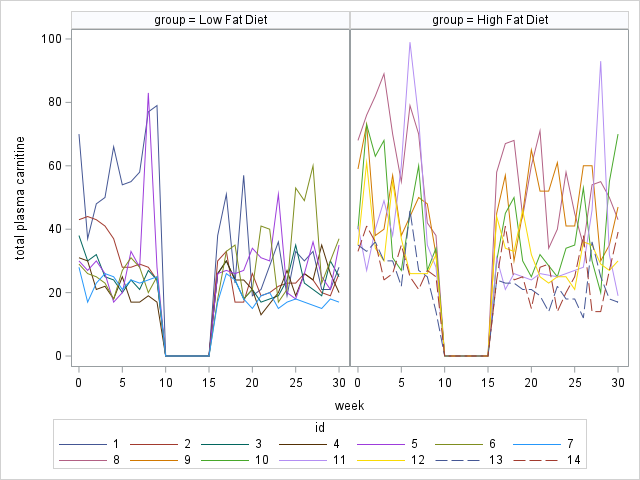
\includegraphics[scale=0.8]{HW4/img/desc1.png}
    \caption{Carnitine Trajectory}
\label{fig:desc1}
\end{figure}

Overall, we could see that the carnitine measurements are higher in group 2, which is high fat diet. And we could see a linear increasing trend between the carnite measurements and time in both groups. 

Second, we would like to see how strong the correlation between the repeated carnitine measurements, and if they are multivariately normally distributed, we can make scatterplot matrices with PROC CORR which also computes means, standard deviations and cross-correlations between the observations at various occations.

The below figure (Figure \ref{fig:desc2}) is the pearson correlation matrix of carnitine measures 0-9. 
\begin{figure}[h]
\centering
\begin{minipage}{.5\textwidth}
  \centering
  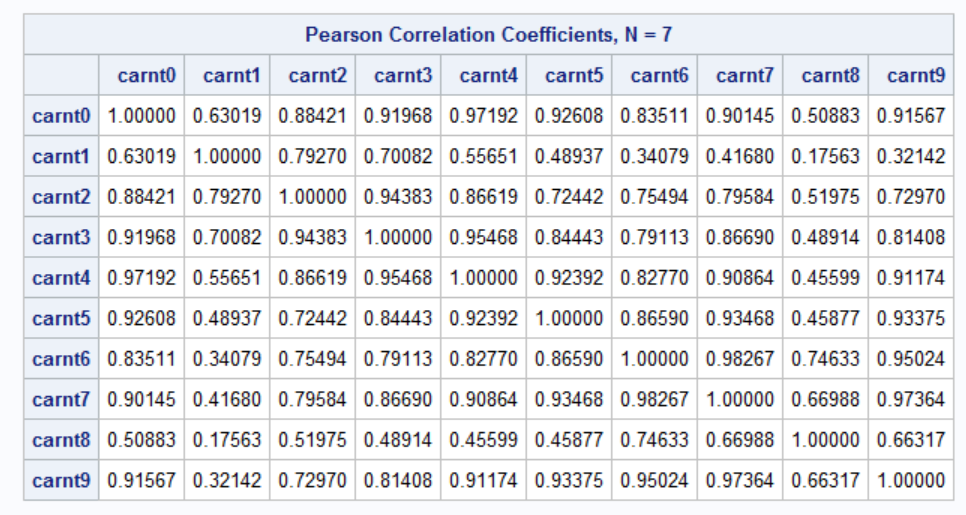
\includegraphics[width=1\linewidth]{HW4/img/desc2.png}
  \captionof{figure}{Correlation}
  \label{fig:test1}
\end{minipage}%
\begin{minipage}{.5\textwidth}
  \centering
  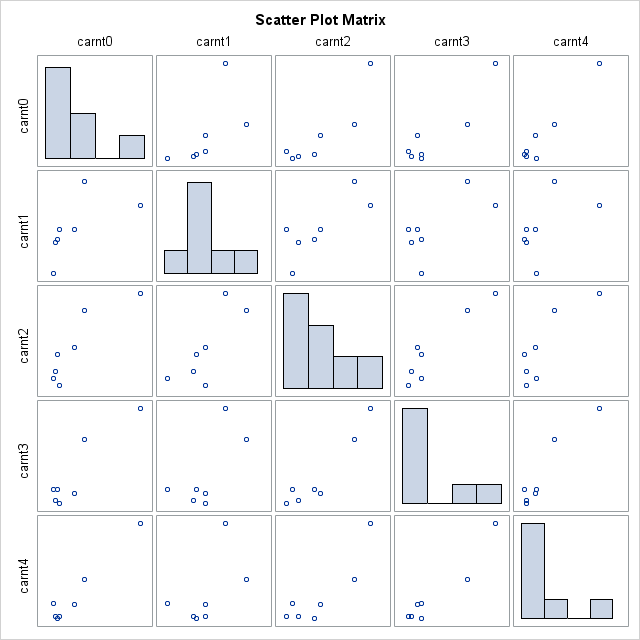
\includegraphics[width=1\linewidth]{HW4/img/desc3.png}
  \captionof{figure}{Histogram}
  \label{fig:test2}
\end{minipage}
   \caption{Pearson Correlation Matrix}
\label{fig:desc2}
\end{figure}

 
From the above correlation matrix, we could see strong correlation between the repeated measurements, which also indicated multivariate normal distribution between them. 

Third, we would like to look at the trend in summary statistics over time. As shown in the below figure (Figure \ref{fig:desc3}), the high fat diet group has higher means than the low fat diet group. Also we can see that the means of carnitine measurements are higher before week 10 than after. We can see the trend that a high, exclusively polyunsaturated, fat diet would decrease the carnitine measurement.

\begin{figure}[h]
    \centering
\textbf{Carnitine Means}\par\medskip
    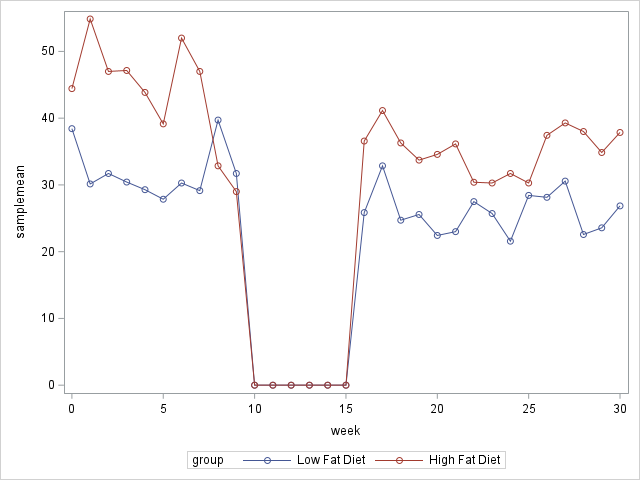
\includegraphics[scale=0.8]{HW4/img/desc4.png}
    \caption{Pearson Correlation Matrix}
\label{fig:desc3}
\end{figure}

								\vspace{0.2cm}
								\item[(B)] It is of interest to explore the differences in total carnitine between the high and low
													 fat diets after adjusting for the baseline carnitine level. Answer this question using
													 the week 9 measurement as the outcome variable. In your report, be sure to do the following:
													 
												\begin{itemize}
													\vspace{0.2cm}
													\item[(i)] Develop an appropriate analysis plan. Write an explicit form for your model.
																		 State any assumptions needed for estimation, inference, and hypothesis testing.

If we uses week 9 carnitine measuremnt as outcome, which is a cross-section analysis. And the model use the baseline measure as a covariate, the model is displayed as below. 
Because it is a randomized trial, the measurement at baseline are considered as the same regardless of group. We will not include the treatment group as a single covariate.

\begin{align*}
Y_{i} &=  \beta_{1} Y_{i0} +  \beta_{2}* I (group= 2) + \epsilon,
\end{align*}

where $Y_{i} $ is the measurement at week 9 for subject i. $Y_{i0}$ is the baseline measurement at week 0 for subject i. 

The assumption of error term is $\epsilon \sim N(0, \sigma^2)$, which means that the errors are i.i.d (independent, identical) Gaussian distribution regardless of group. 

The hypothesis test are:
\begin{align*}
H_0: & \beta_2 = 0 \\
H_1: & \beta_2 \neq 0
\end{align*}

													\vspace{0.2cm}
												  \item[(ii)] Conduct the analysis and provide results.	This includes any diagnostic or sensitivity analyses
																			that you feel are appropriate.
The SAS output results are as below in figure (Figure \ref{fig:b1}):
\begin{figure}[h]
    \centering
    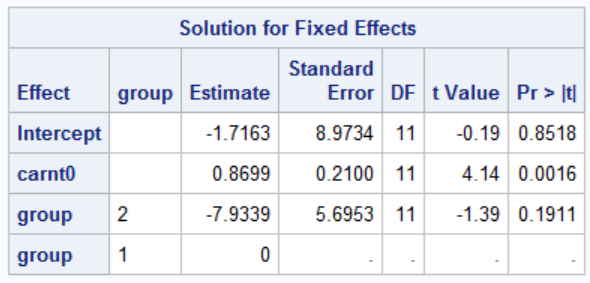
\includegraphics[scale=1]{HW4/img/b1.png}
    \caption{SAS output for B(i)}
\label{fig:b1}
\end{figure}

From the above result, there is no signficant difference in group effect in the week 9 measurement, as p-value for interaction term between group = 0.1911. Instead the baseline measurement is significant which indicates that the baseline measurements effect in week 9 measuremnt is significant. 

From the type III test, we could see that the p-value for interaction terms is 0.39, which we will not reject the null hypothesis, and conclude that there is no siginficant difference in group effect. 

The diagnostic analysis mainly focus on the influential and outlier points. For linear model, we could look at the scaled residual and Cook's distance. The first 5 largest observations with scaled residual and Cook's distance as below.

\begin{minipage}{\linewidth}
\centering
\captionof{table}{Scaled Residual} \label{tab:title} 
\begin{tabular}{@{}p{0.2\textwidth}>{\centering}p{0.2\textwidth}>{\centering\arraybackslash}p{0.5\textwidth} @{} }\toprule[1.5pt]
\bf ID & \bf Group    & \bf Absolute of Scaled Residual \\\midrule
1 & 1 & 1.90746 \\
2       & 1  & 1.125    \\
 8      & 2  &  1.10728   \\
12      & 2  &   1.07807  \\
9 & 2 &  0.93121 \\\midrule
\bottomrule[1.25pt]	
\end {tabular}\par
\bigskip
\end{minipage}

\begin{minipage}{\linewidth}
\centering
\captionof{table}{Cook's D} \label{tab:title} 
\begin{tabular}{@{}p{0.2\textwidth}>{\centering}p{0.2\textwidth}>{\centering\arraybackslash}p{0.5\textwidth} @{} }\toprule[1.5pt]
\bf ID & \bf Group    & \bf Cook's D \\\midrule
1 &  1 & 3.28971 \\
8 & 2 & 0.38030 \\
9 & 2 & 0.11177 \\
12 & 2 & 0.10301 \\
2 & 1 & 0.08871\\
\bottomrule[1.25pt]	
\end {tabular}\par
\bigskip
\end{minipage}

We could see that only subject 1 has large scaled residual and Cook's distance. The Cook's distance is considered high if it is greater than 0.5 and extreme if it is greater than 1. If a point has been flagged by the Cook's distance, the point is considered highly influential and has a combination of unusual explanatory variables and response values. So we will need to do a sensitivity analysis by excluding the observation of subject 1. 

After removing subject 1, both the baseline measurement and group effect are not significant. The SAS output is as below Figure \ref{fig:b3}:
\begin{figure}[h]
    \centering
    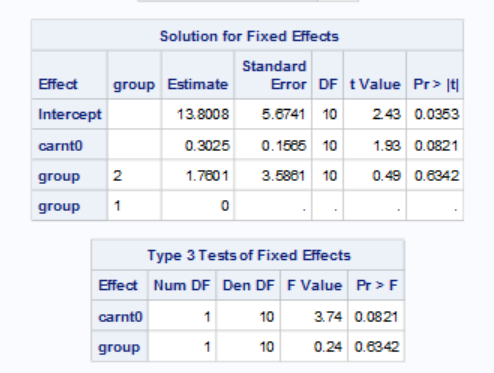
\includegraphics[scale=1]{HW4/img/b1-3.png}
    \caption{Sensitivity Analysis for B(i)}
\label{fig:b3}
\end{figure}

													
													\vspace{0.2cm}
												  \item[(iii)] Provide a summary of your analysis results in language the investigator can understand. All tables 
																			 and figures included in the summary should be accompanied by sufficient exposition to help the 
																			 investigator understand the purpose of the table or figure. 

The mean difference between high fat diet and low fat diet at week 9 of Group 1 is estimated at -7.9339 nmol/ml, which means that the carnitine measurement of high fat diet group is less than low fat diet group by average of 7.9339 nmol/ml. The p-value for testing the difference between two groups is 0.19, which is greater than the significance level 0.05. Therefore, there is no significant evidence that low fat diet group will lead to high carnitine level.
		
											   \end{itemize}
								
								\vspace{0.2cm}
								\item[(C)] Conduct a repeated measures analysis using the first 9 weeks of measurements to study the effect of high 
													 versus low fat diets on total carnitine after adjusting for the baseline carnitine level. In your report, 
													 be sure to include the following:
							
													\begin{itemize}
													\vspace{0.2cm}
													\item[(i)] Develop an appropriate analysis plan. Write an explicit form for your model.
																		 Given the small sample size, discuss relevant assumptions and selection of method needed for estimation, inference, and hypothesis testing.

For repeated measures analysis with random effect model, the measurements within the same subject are correlated, and we assume the variance structure for the repeated measurements is compound symmetry considering small sample size. 

In randomized study, the baseline measurement at week 0 is considered the same regardless of group. So we will not put the single group effect in the model. Also the treatment group will set to "low fat diet" at the time of the baseline. 

The Multiple repeated measurement model is as below:
\begin{align*}
Y_{ij} &=\beta_1 +  \beta_{2} Y_{i0}  + \beta_{3j} I(week = j) + \beta_{4j} I(group=2) I(week =j)  + \epsilon_{ij}
\end{align*}

where $Y_{ij}$ is the measurement at week j for subject i, and the assumption of error term is as below:
\begin{align*}
\epsilon_{ij} & \sim  N(0_{n_i}, \Sigma_{n_{i}*n_{i}}) \\
\Sigma_{n_{i}*n_{i}} &= \begin{pmatrix}
\sigma^2 & \rho \sigma^2 & .. & \rho \sigma^2 \\
..&.. \\
\rho \sigma^2 & \rho \sigma^2 & .. & \sigma^2 \\
\end{pmatrix}
\end{align*}
We assume that the error covariance structure has two components: group effect and random effect of the subject. 

For estimation and hypothesis tesing, REML method was used and the method developed by Kenward and Roger was used for the degree of freedom.

The hypothesis test of difference between group effects are 
\begin{align*}
H_0: & \beta_{41} = \beta_{42} = .. = \beta_{49} = 0 \\
H_1: & \text{ at least one of }\beta_{4j} \neq 0 
\end{align*}



	
													\vspace{0.2cm}
												  \item[(ii)] Conduct the analysis and provide results.	This includes any diagnostic or sensitivity analyses
																			that you feel are appropriate.
The SAS output results are as below in figure (Figure \ref{fig:c1}):
\begin{figure}[h]
    \centering
    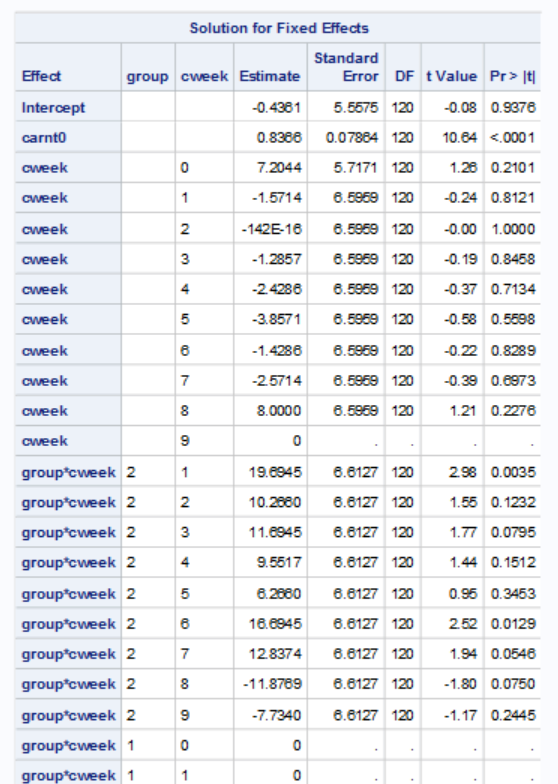
\includegraphics[scale=1]{HW4/img/c1.png}
    \caption{SAS output for C(i)}
\label{fig:c1}
\end{figure}

From the above result, there is signficant difference in group effect in week 1, 6 cartinine measurement, as p-value for interaction term for week 1 is 0.0079, and for week 6 is 0.0193. 
And there are no significant effect for other week time. 

From the type III test shown in Figure (\ref{fig:c2}), we could see that the p-value for interaction terms is < 0.0025, which we will reject the null hypothesis, and conclude that there is siginficant difference in group effect over time. 
\begin{figure}[h]
    \centering
    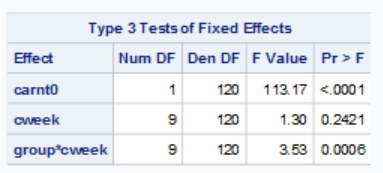
\includegraphics[scale=1]{HW4/img/c2.png}
    \caption{Type III test for C(i)}
\label{fig:c2}
\end{figure}

The diagnostic analysis mainly focus on the scaled residual and Cook's distance. The first 5 largest observations with scaled residual and Cook's distance as below.

\begin{minipage}{\linewidth}
\centering
\captionof{table}{Diagnositic} \label{tab:title} 
\begin{tabular}{@{}p{0.1\textwidth}>{\centering}p{0.1\textwidth}>{\centering}p{0.1\textwidth}>{\centering\arraybackslash}p{0.2\textwidth} @{} }\toprule[1.5pt]
\bf ID & \bf Group  & Week  & \bf Absolute of Scaled Residual \\\midrule
5 & 1 & 8 & 4.07928 \\
11  & 2  & 6 &  4.04129    \\
 11 & 2 & 7   & 2.50155 \\
11   & 2  & 1 &  2.02506  \\
10 & 2 & 3 & 1.99050 \\
\bottomrule[1.25pt]	
\end {tabular}\par
\bigskip
\end{minipage}

The Cook's distance for all the subjects are in Figure (\ref{fig:c3})
\begin{figure}[h]
    \centering
    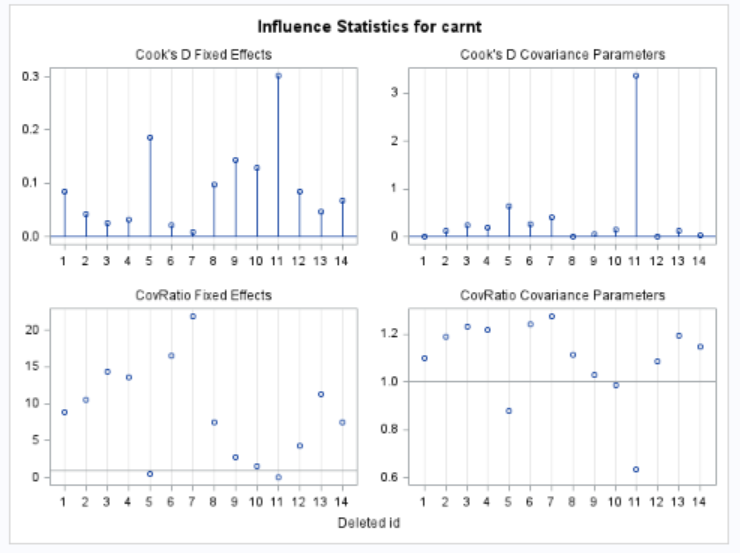
\includegraphics[scale=1]{HW4/img/c3.png}
    \caption{Cook's Distance for C(i)}
\label{fig:c3}
\end{figure}

\begin{minipage}{\linewidth}
\centering
\captionof{table}{Cook's Distance} \label{tab:title} 
\begin{tabular}{@{}p{0.2\textwidth}>{\centering\arraybackslash}p{0.5\textwidth} @{} }\toprule[1.5pt]
\bf ID   & \bf Cook's D \\\midrule
11   & 0.30237 \\
5   & 0.18574\\
9 &  0.14378 \\
10 &   0.12959 \\
8 &   0.09852\\
\bottomrule[1.25pt]	
\end {tabular}\par
\bigskip
\end{minipage}

We could see that all subjects have small Cook's distance, so we don't need to do sensitivity analysis. 
													
													\vspace{0.2cm}
												  \item[(iii)] Provide a summary of your analysis results in language the investigator can understand. All tables 
																			 and figures included in the summary should be accompanied by sufficient exposition to help the 
																			 investigator understand the purpose of the table or figure. 
	
From the above MMRM model, we could see that there is signficant difference in group effect between high fat diet and low fat diet. For example, at week 1, the difference of cartinine level between high fat diet and low fat diet increase after 1 week, which is 24.7143 nmol/ml. And the change of the difference is significant as p-value is 0.0079. Also at week 6, the difference of cartinine level between high fat diet and low fat diet increase after 6 weeks, which is 21.7143 nmol/ml. And the change of the difference is significant as p-value is 0.0193. However, the increasing trend reverses at week 8, the difference between the two groups change to -6.8571 nmol/ml, however it is not siginifcant. 

	
											   \end{itemize}						
							
							
								\vspace{0.2cm}
								\item[(D)] Compare the analyses in parts (B) and (C). Which analysis is more appropriate for this data set? Justify your answer.				
By comparing the analysis above, the repeated measurement model is more appropriate than the cross-sectional analysis. 
		
The results of the two different analysis are different each other. The analysis of the question (B) is equivalent to one way ANOVA model and results in failing to reject the null hypothesis. On the other hand, the repeated measure analysis in the question (C) results in rejecting the null hypothesis by using linear mixed model.

The repeated measure analysis is more appropriate for this data, because the repeated measure analysis takes into account of the repeated measurement in week 1-9 whereas the one way ANOVA model compares only the end points of two groups. The MMRM model increase the power for detecting the difference between groups by assigning appropriate covariance structure for the error terms. 
							
								\vspace{0.2cm}
								\item[(E)] We are also interested in investigating whether there is an impact of ``switch-over'' from polyunsaturated fat 
													 to saturated fat on the carnitine levels and whether the impact is different for the high fat and low fat diets. 
													 To address these issues, perform an analysis using all available measurements. Baseline carnitine should be 
													 adjusted for in the analysis. In your report, be sure to include the following:
							
													\begin{itemize}
													\vspace{0.2cm}
													\item[(i)] Develop an appropriate analysis plan. Write an explicit form for your model.
																		 State any assumptions needed for estimation, inference, and hypothesis testing.

We will build up a random effect mixed model, including week as continuous variable, also ajusting for the baseline measurement. The random effect error structure $b_i$ for 

\begin{align*}
Y_{ij} | b_i &=\beta_1 +  \beta_{2} Y_{i0}  + \beta_{3} Time_{j} + \beta_{4} I(group=2) Time_{j}  + \beta_{5} I(diet=2) Time_{j} + + \beta_{6} I(group=2) I(diet=2)Time_{j}  + b_i + \epsilon_{ij} \\
Var(b_i) &= \sigma_b^2, \qquad b_i \sim N(0_{n_i}, \sigma_b^2I_{n_i \times n_i}) \\
Var(\epsilon_{ij}) &= \sigma^2 , \qquad \epsilon_{ij} \sim N(0, \sigma^2 I)
\end{align*}

	
													\vspace{0.2cm}
												  \item[(ii)] Conduct the analysis and provide results.	This includes any diagnostic or sensitivity analyses
																			that you feel are appropriate.
The SAS output results are as below in figure (Figure \ref{fig:e1}):
\begin{figure}[h]
    \centering
    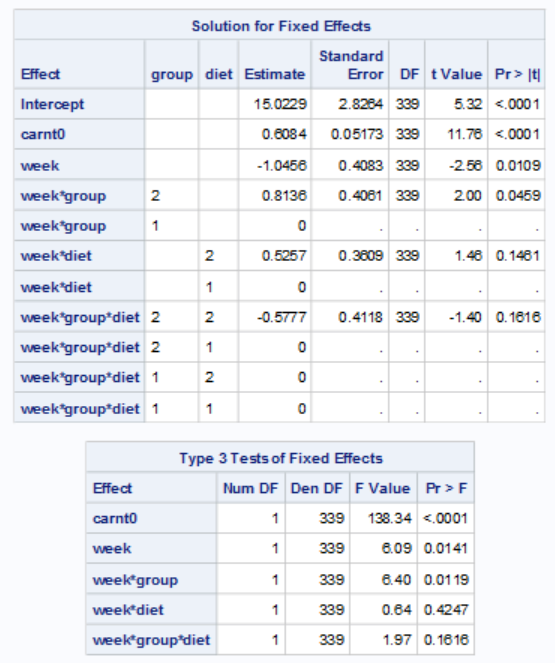
\includegraphics[scale=1]{HW4/img/e1.png}
    \caption{SAS output for E(i)}
\label{fig:e1}
\end{figure}

From the above result, there are signficant effects in baseline measure, week and group effects, as p-value for baseline is < 0.0001, baseline measurement is p < 0.0001, and for week is p = 0.01. The p-value for interaction term of week and group is p= 0.045.

From the type III test shown in Figure (\ref{fig:e1}), we could see that the p-value for interaction terms is p= 0.0119, which we will reject the null hypothesis, and conclude that there is siginficant difference in group effect over time. However, there is no significant effect in diet (unsaturated vs. saturated) over time, as the p-values are > 0.05. 

The diagnostic analysis mainly focus on the scaled residual and Cook's distance. The first 5 largest observations with scaled residual and Cook's distance as below.

\begin{minipage}{\linewidth}
\centering
\captionof{table}{Diagnositic} \label{tab:title} 
\begin{tabular}{@{}p{0.1\textwidth}>{\centering}p{0.1\textwidth}>{\centering}p{0.1\textwidth}>{\centering\arraybackslash}p{0.2\textwidth} @{} }\toprule[1.5pt]
\bf ID & \bf Group  & Week  & \bf Absolute of Scaled Residual \\\midrule
11 & 2 & 28 & 4.78947 \\
11  & 2  & 6 &  4.74559   \\
5 & 1 & 8   & 4.56222 \\
6   & 1  & 27 &  3.24912 \\
10 & 2 & 30 & 3.07549 \\
\bottomrule[1.25pt]	
\end {tabular}\par
\bigskip
\end{minipage}

The Cook's distance for all the subjects are in Figure (\ref{fig:e3})
\begin{figure}[h]
    \centering
    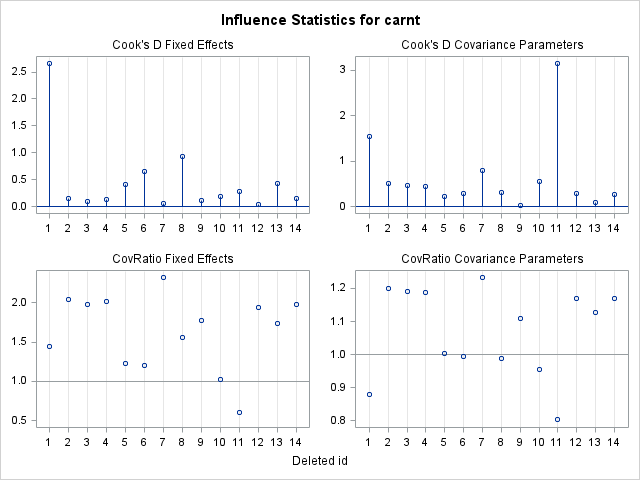
\includegraphics[scale=1]{HW4/img/e3.png}
    \caption{Cook's Distance for E(i)}
\label{fig:e3}
\end{figure}

\begin{minipage}{\linewidth}
\centering
\captionof{table}{Cook's Distance} \label{tab:title} 
\begin{tabular}{@{}p{0.2\textwidth}>{\centering\arraybackslash}p{0.5\textwidth} @{} }\toprule[1.5pt]
\bf ID   & \bf Cook's D \\\midrule
1   & 2.65981 \\
8  & 0.93989\\
6 &  0.65560 \\
13 &  0.43009 \\
5 &   0.40675\\
\bottomrule[1.25pt]	
\end {tabular}\par
\bigskip
\end{minipage}
				
We could see that the subject 1 has influenced the analysis result with Cook's Distance 2.66, so we will do a sensitivity analysis by removing subject 1 and the SAS output is as below Figure (\ref{fig:e4}):

\begin{figure}[h]
    \centering
    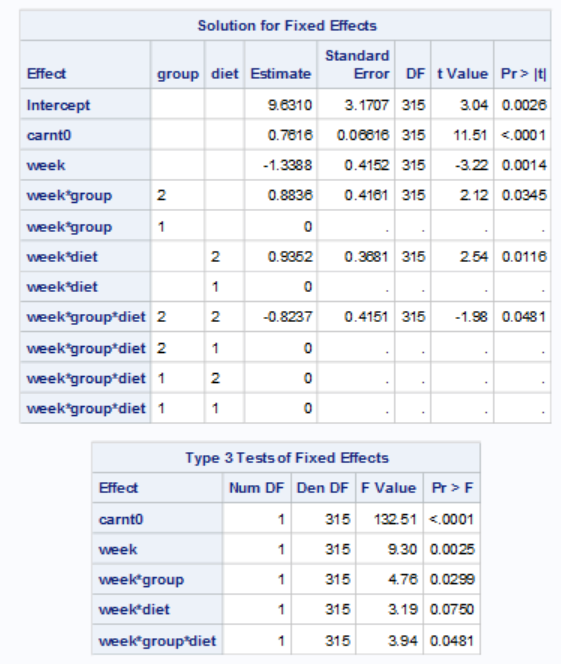
\includegraphics[scale=1]{HW4/img/e4.png}
    \caption{Sensitivity Analysis for E(i)}
\label{fig:e4}
\end{figure}
			
We could see that, after removing subject 1, both group and interaction of group and diet effects are significant with p-value = 0.03 and 0.0481. 
						
													\vspace{0.2cm}
												  \item[(iii)] Provide a summary of your analysis results in language the investigator can understand. All tables 
																			 and figures included in the summary should be accompanied by sufficient exposition to help the 
																			 investigator understand the purpose of the table or figure. 

By removing the influential subject 1 from the above linear mixed model with random effect analysis, we found that there is signficant effect of group and interaction of group and fat saturation, besides baseline covariates. It shows that the mean difference of cartinine measurements in high fat and low fat group changes significantly with time. And the mean difference of cartinine between saturated fat and unsaturated also changes signficantly different within high fat and low fat group. 

		
											   \end{itemize}								

   \end{itemize}	
				
\newpage


	\noindent \textbf{Problem 2} -- Adults with intellectual and developmental disabilities (IDD) are living longer, and an
																	increasing number are now living and working in the community instead of residing in
																	institutions. Because of the increasing number of middle-aged and older persons with IDD,
																	there is growing concern about cardiovascular disease (CVD) in the IDD population. This
																	concern is due to a number of studies showing that conditions related to CVD may be
																	more prevalent in the IDD population and may affect persons with IDD at a younger age
																	than in the general population. \\
																	
																	\vspace{0.2cm}
																	UNC investigators plan to collect data on adults with mild to moderate IDD served
																	by compensatory education programs in North Carolina community colleges. In a pilot
																	study, they learned that IDD adults had HDL (``good'') cholesterol levels much lower
																	than those in the general population. They plan to conduct a study in 5 community
																	colleges to determine whether a walking for exercise intervention can be used to increase
																	HDL cholesterol levels among IDD adults. Within each community college, 100 adults
																	with IDD will be randomized to two groups, each with 50 adults: walking for exercise, or
																	placebo. Each subject will have HDL cholesterol measured at $t=0$ months (baseline), $t=6$ months,
																	and $t=12$ months. (Walking has been shown to be an effective way to increase
																	HDL cholesterol to healthy levels.) \\
																	
																	\vspace{0.2cm}
																	The investigators will fit the linear mixed effects model for subject $i$ in college $h$ at month
																	$t$:
																	\[
																			Y_{hit} = \beta_0 + \beta_1t + \beta_2 t x_{hi} + u_h + b_{hi} + \epsilon_{hit},
																	\]
																	where $\epsilon_{hit} \overset{iid}{\sim} \text{N}\left(0,\sigma^2_e\right)$ independent of 
																	$b_{hi} \overset{iid}{\sim} \text{N}\left(0,\sigma^2_b\right)$ independent of 
																	$u_{h} \overset{iid}{\sim} \text{N}\left(0,\sigma^2_h\right)$. The variable $x_{hi} = 1$
																	if the participant is randomized to the walking exercise group and $x_{hi} = 0$ if randomized
																	to placebo.
																	%
																	Integrating over the random effects, they expect that the marginal distribution of $Y_{hit}$ (mg/dL HDL cholesterol) 
																	in the control group would be approximately normally distributed with mean $50$ and variance $13^2$. They would like to 
																	know the minimum detectable effect of the walking program (measured by $\beta_2$) for a linear time trend  
																	assuming that $\beta_0$ = 50 and $\beta_1 = 0.01667$, using a 2-sided test with type I error 
																	rate of 5\% and power equal to 80\%. For the error structure, they assume that observations on the same adult should have 
																	correlation 0.60 regardless of their spacing in time and that observations on different adults at the same community college 
																	should have correlation 0.20. \\
																	
								\begin{itemize}
								\vspace{0.2cm} 
								\item[(A)] Clearly describe the steps you will take to calculate the minimum (absolute) detectable value of $\beta_2$ for the study above, providing all
								           important details regarding the simulation study performed. Give the values of the variance components implied by the information provided. 	

\begin{align*}
Y_{hit} &= \beta_0 + \beta_1t + \beta_2 t x_{hi} + u_h + b_{hi} + \epsilon_{hit},
\end{align*}

The error structure of control group is combination of control group measurement error and random effect of subject and community. For the same subject with different observations:
\begin{align*}
\epsilon_{hit} \overset{iid}{\sim} \text{N}\left(0,\sigma^2_e\right) \\
b_{hi} \overset{iid}{\sim} \text{N}\left(0,\sigma^2_b\right)\\
u_{h} \overset{iid}{\sim} \text{N}\left(0,\sigma^2_h\right)\\
Cov(Y_{hit_1}, Y_{hit_2}) &=Cov( \beta_0 + \beta_1t + \beta_2 t x_{hi} + u_h + b_{hi} + \epsilon_{hit},  \beta_0 + \beta_1t + \beta_2 t x_{hi} + u_h + b_{hi} + \epsilon_{hit})  \\ 
&=Var(u_h) + Var(b_{hi}) + Cov(\epsilon_{hit_1}, \epsilon_{hit_2}), \qquad Cov(\epsilon_{hit_1}, \epsilon_{hit_2}) = 0 \\
&= \sigma^2_b + \sigma^2_h \\
&= 0.8 \sigma_e^2\\
Var(Y_{hit}) &= \sigma^2_b + \sigma^2_h +  \sigma_e^2 = 1.8 \sigma_e^2\\
\Sigma_{hi} &= \begin{pmatrix}
1.8 \sigma_e^2  &.. & 0.8 \sigma_e^2\\
0.8 \sigma_e^2 &..& 1.8 \sigma_e^2\\
&.. & \\
0.8 \sigma_e^2 & .. &.. & 1.8 \sigma_e^2\\
\end{pmatrix}
\end{align*}

For different subjects in the same community, they are correlated at the community level.
\begin{align*}
Cov(Y_{hit}, Y_{hjt})  &=Cov( \beta_0 + \beta_1t + \beta_2 t x_{hi} + u_h + b_{hi} + \epsilon_{hit},  \beta_0 + \beta_1t + \beta_2 t x_{hi} + u_h + b_{hi} + \epsilon_{hit})  \\ 
&=Var(u_h) + Cov(\epsilon_{hit}, \epsilon_{hjt}) \\
& =  \sigma^2_h = 0.2 \sigma_e^2
\end{align*}

For different subjects in different community, they are independent
\begin{align*}
Cov(Y_{h_1it}, Y_{h_2jt})  &=Cov( \beta_0 + \beta_1t + \beta_2 t x_{h_{1i}} + u_{h1} + b_{h_1i} + \epsilon_{h_1it},  \beta_0 + \beta_1t + \beta_2 t x_{h_{2i}} + u_{h2} + b_{h_1i} + \epsilon_{h_2it})  \\ 
&=0 
\end{align*}

So we have the MVN distributions of control and walking group with covariance structure of $\Sigma$
\begin{align*}
\Sigma &= \begin{pmatrix} 
\Sigma_{hi} &  0.2 \sigma_e^2 &.. & 0 \\
 0.2 \sigma_e^2 &\Sigma_{hi} &..& 0 \\
..&..\\
 0 &.. & 0.2 \sigma_e^2 &\Sigma_{hi} \\
\end{pmatrix}
\end{align*}

When $\beta_0, \beta_1$ are known, the variance of $\hat{\beta}_2$ are
\begin{align*}
Var(\hat{\beta}_2)&= \big( \sum_{j=1}^n (t_j - \bar{t})^2 \big)^{-1} \sigma_e^2 + \sigma_h^2 + \sigma_b^2 \\
 \bar{t} &= \frac{1}{n} \sum_{j=1}^n t_j
\end{align*}

Then we have the distribution for $\beta_2$ is 

\begin{align*}
\beta_2 & \sim N(0, Var(\hat{\beta}_2)) \\
Var(\hat{\beta}_2)&= \big( \sum_{j=1}^n (t_j - \bar{t})^2 \big)^{-1} \sigma_e^2 + \sigma_h^2 + \sigma_b^2 \\
\sigma_{\beta}^2 &=\big[ \big( \sum_{j=1}^n (t_j - \bar{t})^2 \big)^{-1} + 0.8 \big ] \sigma_e^2  \\
\sum_{j=1}^n (t_j - \bar{t})^2 &= \big(\tau^2 n(n+1) \big)/ \big(12(n-1) \big) , \quad \tau \text{is duration of the study} \\
\sigma_{\beta}^2 &= 135.3
\end{align*}

First step, simulation of possible $\beta_2$ ranging from 0 to a certain number $b$, get the walking group $\beta_2$ distributions.
The control group $\beta_2$ distribution could be considered as $N(0, Var(\beta_2))$. 

Second step: Found the $\delta$ that falls in the rejection region of control group distribution with $5\%$ of the time. Then we will find the minimual detectable $\delta$ falls into the walking group distribution with probability $80\%$. 

\begin{align*}
\alpha &= Pr(\text{Reject } H_0 | H_0 \text{ is true} ) \\ 
\text{Power} &= Pr(\text{Reject } H_0 | H_0 \text{ is false})
\end{align*}




								\vspace{0.2cm} 
								\item[(B)] Provide the minimum detectable $\beta_2$ if the investigators carry out the study in 5 North Carolina community colleges, randomizing exactly
													 50 adults to placebo and 50 adults to the walking intervention within each community college. Assume that follow-up rates are 100\% (i.e., no missing data).


By simulation, the $\delta = 32.6$, and the R codes are as below
\lstinputlisting[language=R]{HW4/BIOS767_hw4.rmd}


								\vspace{0.2cm} 
								\item[(C)] Investigators may gain additional financial support, which they could use to (i) double the number of community colleges from 5 to 10, keeping 100 adults in 
													 each, (ii) double the number of adults recruited within each community college, so retaining 5 colleges with 200 subjects each, or (iii) double the number of 
													 follow-up visits of the existing subjects (to approximately 0, 2.4, 4.8, 7.2, 9.6, and 12 months). Advise investigators regarding which approach is optimal 
													 (with respect to having the smallest detectable $\beta_2$ in absolute value) under the setup above. Provide statistical evidence to support your advice. Optimal
													 solutions will produce a graphic of the power function ($\beta_2$ on the x-axis, power and the y-axis).


Then the sample size N for confidence level $\alpha$ and power $1- \gamma$:
\begin{align*}
N &= \frac{\big(Z_{1-\alpha/2} + Z_{1-\gamma}\big)^2 \sigma_{\beta}^2}{\pi (1- \pi) \delta^2}\\
\sigma_{\beta}^2 &= \big( \sum_{j=1}^n (t_j - \bar{t})^2 \big)^{-1} \sigma_e^2 + \sigma_h^2 + \sigma_b^2 \\
\sigma_h^2 &= 0.2 \sigma_e^2, \qquad \sigma_b^2 = 0.6 \sigma_e^2 \\
\sigma_{\beta}^2 &=\big[ \big( \sum_{j=1}^n (t_j - \bar{t})^2 \big)^{-1} + 0.8 \big ] \sigma_e^2 
\end{align*}

Also we can get the formula for $\delta$
\begin{align*}
\delta &= \sqrt{ \frac{\big(Z_{1-\alpha/2} + Z_{1-\gamma}\big)^2 \sigma_{\beta}^2}{\pi (1- \pi) N}} \\
&=  \sqrt{ \frac{\big(Z_{0.975} + Z_{0.8}\big)^2 \sigma_{\beta}^2}{0.5 (1- 0.5) * N}} 
\end{align*}	

From above formula for effect size, the optimal solution is (ii) increasing the number of adults recruited within each college. In this way, we could get such smaller minimum detectable effect with doubled total number. While the (i) would increase the $\sigma_{\beta}^2$ by increasing the community size, and (iii) increase the number of follow-up visits, it would decrease the variance for measurement error, however it won't decrease the $\delta$ as much as in (ii).

The simulation of the power as the change of $\beta_2$ as shown in the figure.
When increase the sample size in each community, and total number is 200
\begin{align*}
\sigma_{\beta}^2 &=\big[ \big( \sum_{j=1}^n (t_j - \bar{t})^2 \big)^{-1} + 0.8 \big ] \sigma_e^2 \\
\sum_{j=1}^n (t_j - \bar{t})^2 &= \big(\tau^2 n(n+1) \big)/ \big(12(n-1) \big) , \quad \tau \text{is duration of the study} \\
&= \big(12^2 200 (200+1) \big)/ \big(12( 200-1) \big) \\
&= 2424\\
\sigma_{\beta}^2 &= \big[ (2424 )^{-1} + 0.8 \big ] \sigma_e^2 \\
&= 0.8\sigma_e^2
\delta &= \sqrt{ \frac{\big(Z_{0.975} + Z_{0.8}\big)^2 \sigma_{\beta}^2}{0.5 (1- 0.5) * N}}  \\
&=  \sqrt{ \frac{\big(1.96 + 0.86 \big)^2* 0.8 * 13^2}{0.5 (1- 0.5) * 200}} \\
&= 21.5
\end{align*}

When increase the number of communities from 5 to 10, 
\begin{align*}
\sigma_{\beta}^2 &= 135.3\\
\delta &= \sqrt{ \frac{\big(Z_{0.975} + Z_{0.8}\big)^2 \sigma_{\beta}^2}{0.5 (1- 0.5) * N}}  \\
&=  \sqrt{ \frac{\big(1.96 + 0.86 \big)^2 135.3}{0.5 (1- 0.5) * 200}} \\
&= 
\end{align*}






								\vspace{0.2cm} 
								\item[(D)] Assuming the investigators use the setup in part (a), they wish to conduct a power calculation that accommodates missing data. Suppose that the missing data satisfy 
													 monotone dropout are otherwise generated as follows. Let $R_{hit}=1$ indicate that $Y_{hit}$ is missing (and hence all future measurements).
														\[
																 \text{logit}\left[\text{P}\left( R_{hit} = 1 \big|  \mathbf{Y}_{hi}\right)\right] = 3.95 - 0.09 \cdot Y_{hi,t-1},
														\]
													 for $t>0$ and that all participants have an observed value of $Y_{hit}$ at time $t=0$. Are the missing data MCAR, MAR, or NMAR in this case? Is it meaningful 
													 to consider the power of the test in this setting? Explain. If it is meaningful, what is the minimum detectable value of $\beta_2$?

It is NMAR, not missing at random. As the logit probabililty of missing is based on previous observation, which indicates that the missing probability is associated with observed data, so it is not missing at random.




													 \end{itemize}
							

